\chapter{Equation(s) of Motion}
This chapter elaborates mathematical definition and generalized nonlinear equations of motion of a rigid spacecraft equipped with array of SGCMG units.

\section{Kinematics}
\subsection{Euler Angles}
\subsection{Quaternions}
Quaternion is a commonly used 3D rotation parameterization. It is written like $\mathbf{q}=q_0 + q_1 i + q_2 j + q_3 k$, in which $i, j, k$ forms the three bases of the imaginary part (analogous to the imaginary part of a complex number) and $i^2=j^2=k^2=-1$. Usually a rotation is represented by a unit quaternion (a quaternion whose norm is 1).
\[i^2=j^2=k^2=ijk=-1\]

\[{\bf R}=\begin{bmatrix} 1-2q_2^2-2q_3^2 & 2q_1q_2-2q_0q_3 & 2q_1q_3+2q_0q_2 \\ 2q_1q_2+2q_0q_3 & 1-2q_1^2-2q_3^2 & 2q_2q_3-2q_0q_1 \\ 2q_1q_3-2q_0q_2 & 2q_2q_3+2q_0q_1 & 1-2q_1^2-2q_2^2 \end{bmatrix}\]

while JPL defines

\[i^2=j^2=k^2=ijk=1\]


\section{Dynamics}
\subsection{System Identification}
\subsection{CMG Modeling}

\begin{figure}[!h]
    \centering
    \tikzset{every picture/.style={line width=0.75pt}} %set default line width to 0.75pt        

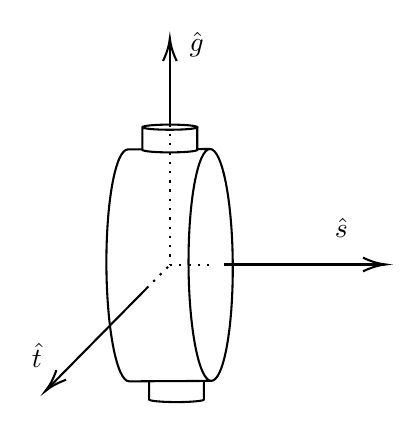
\begin{tikzpicture}[x=0.75pt,y=0.75pt,yscale=-1,xscale=1]
%uncomment if require: \path (0,249); %set diagram left start at 0, and has height of 249

%Shape: Can [id:dp06527002916107127] 
\draw  [fill={rgb, 255:red, 255; green, 255; blue, 255 }  ,fill opacity=1 ] (342.4,199.14) -- (342.4,210.05) .. controls (342.4,210.73) and (336.49,211.29) .. (329.2,211.29) .. controls (321.91,211.29) and (316,210.73) .. (316,210.05) -- (316,199.14) .. controls (316,198.46) and (321.91,197.9) .. (329.2,197.9) .. controls (336.49,197.9) and (342.4,198.46) .. (342.4,199.14) .. controls (342.4,199.82) and (336.49,200.38) .. (329.2,200.38) .. controls (321.91,200.38) and (316,199.82) .. (316,199.14) ;
%Shape: Can [id:dp8096689677898681] 
\draw  [color={rgb, 255:red, 0; green, 0; blue, 0 }  ,draw opacity=1 ][fill={rgb, 255:red, 255; green, 255; blue, 255 }  ,fill opacity=1 ] (345.97,201.08) -- (306.4,201.3) .. controls (300.52,201.33) and (295.61,176.35) .. (295.43,145.49) .. controls (295.26,114.64) and (299.89,89.6) .. (305.78,89.57) -- (345.34,89.35) .. controls (351.23,89.31) and (356.14,114.3) .. (356.31,145.15) .. controls (356.48,176.01) and (351.85,201.04) .. (345.97,201.08) .. controls (340.08,201.11) and (335.17,176.12) .. (335,145.27) .. controls (334.83,114.42) and (339.46,89.38) .. (345.34,89.35) ;
%Shape: Can [id:dp5210820858304941] 
\draw  [fill={rgb, 255:red, 255; green, 255; blue, 255 }  ,fill opacity=1 ] (339.2,78.84) -- (339.2,89.75) .. controls (339.2,90.43) and (333.29,90.99) .. (326,90.99) .. controls (318.71,90.99) and (312.8,90.43) .. (312.8,89.75) -- (312.8,78.84) .. controls (312.8,78.16) and (318.71,77.6) .. (326,77.6) .. controls (333.29,77.6) and (339.2,78.16) .. (339.2,78.84) .. controls (339.2,79.53) and (333.29,80.08) .. (326,80.08) .. controls (318.71,80.08) and (312.8,79.53) .. (312.8,78.84) ;
%Straight Lines [id:da7302123237400429] 
\draw  [dash pattern={on 0.84pt off 2.51pt}]  (314.87,156.42) -- (326,145.29) ;
%Straight Lines [id:da6678919295963763] 
\draw  [dash pattern={on 0.84pt off 2.51pt}]  (326,145.29) -- (348,145.29) ;
%Straight Lines [id:da12300205948280718] 
\draw  [dash pattern={on 0.84pt off 2.51pt}]  (326,77.6) -- (326,145.29) ;
%Straight Lines [id:da7145265678364978] 
\draw    (352,145) -- (428,145) ;
\draw [shift={(430,145)}, rotate = 180] [color={rgb, 255:red, 0; green, 0; blue, 0 }  ][line width=0.75]    (10.93,-3.29) .. controls (6.95,-1.4) and (3.31,-0.3) .. (0,0) .. controls (3.31,0.3) and (6.95,1.4) .. (10.93,3.29)   ;
%Straight Lines [id:da06879773433820491] 
\draw    (314.87,156.42) -- (267.4,204.58) ;
\draw [shift={(266,206)}, rotate = 314.59000000000003] [color={rgb, 255:red, 0; green, 0; blue, 0 }  ][line width=0.75]    (10.93,-3.29) .. controls (6.95,-1.4) and (3.31,-0.3) .. (0,0) .. controls (3.31,0.3) and (6.95,1.4) .. (10.93,3.29)   ;
%Straight Lines [id:da9989157109226341] 
\draw    (326,77.6) -- (326,38) ;
\draw [shift={(326,36)}, rotate = 450] [color={rgb, 255:red, 0; green, 0; blue, 0 }  ][line width=0.75]    (10.93,-3.29) .. controls (6.95,-1.4) and (3.31,-0.3) .. (0,0) .. controls (3.31,0.3) and (6.95,1.4) .. (10.93,3.29)   ;

% Text Node
\draw (404,121.4) node [anchor=north west][inner sep=0.75pt]    {$\hat{s}$};
% Text Node
\draw (334,31.4) node [anchor=north west][inner sep=0.75pt]    {$\hat{g}$};
% Text Node
\draw (258,181.4) node [anchor=north west][inner sep=0.75pt]    {$\hat{t}$};

\end{tikzpicture}
    \caption{Axis definition for Control Moment Gyroscope}
    \label{fig:tikCMG}
\end{figure}

\begin{figure}[!h]
    \centering
    

\tikzset{every picture/.style={line width=0.75pt}} %set default line width to 0.75pt        

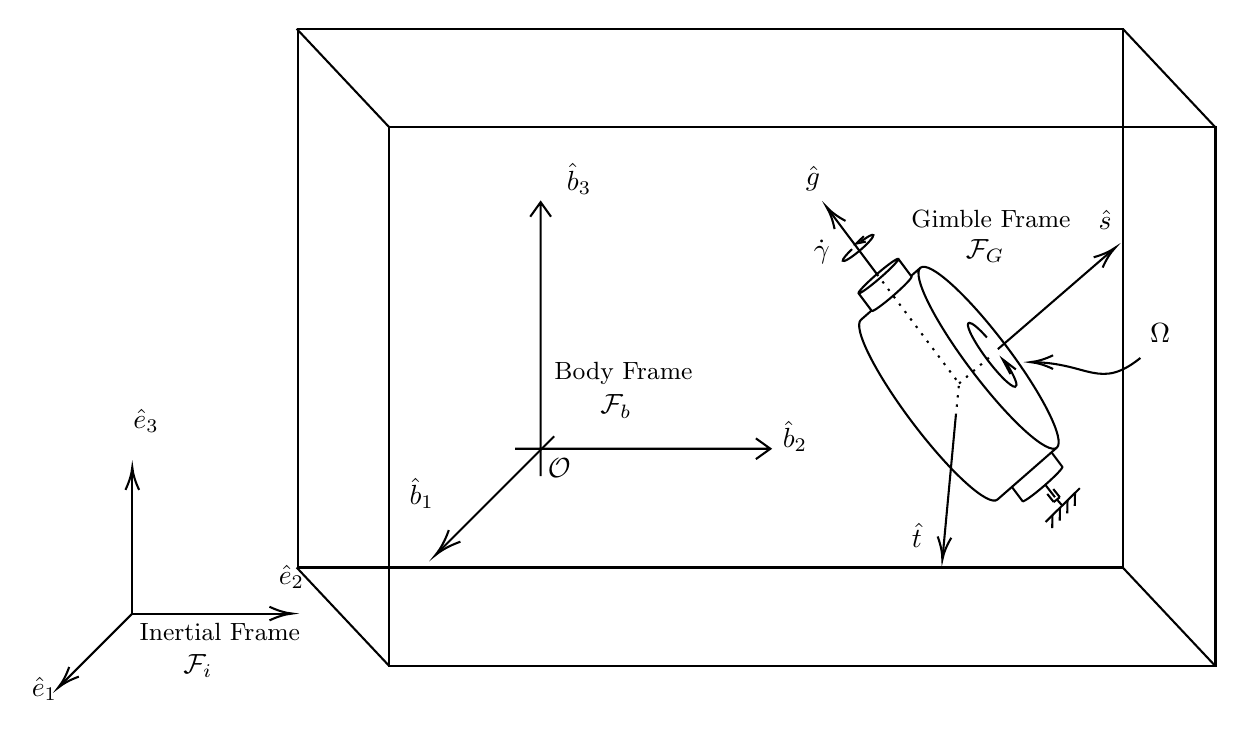
\begin{tikzpicture}[x=0.75pt,y=0.75pt,yscale=-1,xscale=1]
%uncomment if require: \path (0,356); %set diagram left start at 0, and has height of 356

%Shape: Can [id:dp8331189729524409] 
\draw  [fill={rgb, 255:red, 255; green, 255; blue, 255 }  ,fill opacity=1 ] (494.82,207.43) -- (501.2,215.92) .. controls (501.6,216.46) and (497.63,220.59) .. (492.34,225.17) .. controls (487.05,229.74) and (482.44,233.02) .. (482.04,232.49) -- (475.66,223.99) .. controls (475.26,223.46) and (479.23,219.32) .. (484.52,214.75) .. controls (489.81,210.17) and (494.42,206.9) .. (494.82,207.43) .. controls (495.22,207.96) and (491.25,212.1) .. (485.97,216.67) .. controls (480.68,221.25) and (476.06,224.52) .. (475.66,223.99) ;
%Shape: Can [id:dp8805062966141313] 
\draw  [color={rgb, 255:red, 0; green, 0; blue, 0 }  ,draw opacity=1 ][fill={rgb, 255:red, 255; green, 255; blue, 255 }  ,fill opacity=1 ] (498.54,206.7) -- (469.96,231.69) .. controls (465.71,235.41) and (447.54,219.03) .. (429.38,195.12) .. controls (411.22,171.2) and (399.94,148.79) .. (404.19,145.08) -- (432.77,120.08) .. controls (437.02,116.37) and (455.19,132.74) .. (473.35,156.66) .. controls (491.51,180.58) and (502.79,202.99) .. (498.54,206.7) .. controls (494.29,210.42) and (476.12,194.04) .. (457.96,170.12) .. controls (439.79,146.21) and (428.52,123.8) .. (432.77,120.08) ;
%Shape: Can [id:dp6975809963098918] 
\draw  [fill={rgb, 255:red, 255; green, 255; blue, 255 }  ,fill opacity=1 ] (422.17,115.76) -- (428.54,124.26) .. controls (428.94,124.79) and (424.98,128.93) .. (419.69,133.5) .. controls (414.4,138.07) and (409.79,141.35) .. (409.39,140.82) -- (403.01,132.32) .. controls (402.61,131.79) and (406.58,127.65) .. (411.86,123.08) .. controls (417.15,118.5) and (421.77,115.23) .. (422.17,115.76) .. controls (422.57,116.29) and (418.6,120.43) .. (413.31,125.01) .. controls (408.02,129.58) and (403.41,132.86) .. (403.01,132.32) ;
%Straight Lines [id:da7548151699735375] 
\draw  [dash pattern={on 0.84pt off 2.51pt}]  (449.87,191.43) -- (451.44,175.78) ;
%Straight Lines [id:da4676995296398143] 
\draw  [dash pattern={on 0.84pt off 2.51pt}]  (451.44,175.78) -- (467.4,161.98) ;
%Straight Lines [id:da24364084418605625] 
\draw  [dash pattern={on 0.84pt off 2.51pt}]  (411.86,123.08) -- (451.44,175.78) ;
%Straight Lines [id:da603601196492777] 
\draw    (470.13,159.25) -- (525.21,111.62) ;
\draw [shift={(526.73,110.31)}, rotate = 499.15] [color={rgb, 255:red, 0; green, 0; blue, 0 }  ][line width=0.75]    (10.93,-3.29) .. controls (6.95,-1.4) and (3.31,-0.3) .. (0,0) .. controls (3.31,0.3) and (6.95,1.4) .. (10.93,3.29)   ;
%Straight Lines [id:da39680954875025143] 
\draw    (449.87,191.43) -- (443.58,258.71) ;
\draw [shift={(443.39,260.7)}, rotate = 275.34000000000003] [color={rgb, 255:red, 0; green, 0; blue, 0 }  ][line width=0.75]    (10.93,-3.29) .. controls (6.95,-1.4) and (3.31,-0.3) .. (0,0) .. controls (3.31,0.3) and (6.95,1.4) .. (10.93,3.29)   ;
%Straight Lines [id:da931335338150046] 
\draw    (411.86,123.08) -- (388.74,92.28) ;
\draw [shift={(387.54,90.68)}, rotate = 413.1] [color={rgb, 255:red, 0; green, 0; blue, 0 }  ][line width=0.75]    (10.93,-3.29) .. controls (6.95,-1.4) and (3.31,-0.3) .. (0,0) .. controls (3.31,0.3) and (6.95,1.4) .. (10.93,3.29)   ;
%Straight Lines [id:da06748543672273133] 
\draw    (509.61,226.25) -- (493.14,242.49) ;
%Straight Lines [id:da33848315956607067] 
\draw    (492.86,224.43) -- (497.64,230.56) ;
%Straight Lines [id:da9582167503794932] 
\draw    (500.06,235.67) -- (499.93,241.9) ;
%Straight Lines [id:da1212417766847036] 
\draw    (496.44,239.24) -- (496.31,245.48) ;
%Straight Lines [id:da09420728047826432] 
\draw    (507.3,228.52) -- (507.18,234.76) ;
%Straight Lines [id:da8325536037855037] 
\draw    (503.68,232.09) -- (503.56,238.33) ;
%Shape: Rectangle [id:dp2711095269864183] 
\draw   (133,4.86) -- (530.27,4.86) -- (530.27,264.43) -- (133,264.43) -- cycle ;
%Shape: Rectangle [id:dp9597125724935636] 
\draw   (177,52.43) -- (575,52.43) -- (575,312) -- (177,312) -- cycle ;
%Straight Lines [id:da6047312216963134] 
\draw    (132.27,4.86) -- (177,52.43) ;
%Straight Lines [id:da614844554115443] 
\draw    (530.27,4.86) -- (575,52.43) ;
%Straight Lines [id:da9657702374196164] 
\draw    (132.27,264.43) -- (177,312) ;
%Straight Lines [id:da4943938352124151] 
\draw    (530.27,264.43) -- (575,312) ;
%Shape: Axis 2D [id:dp8483204934107569] 
\draw  (237.54,207.23) -- (360.54,207.23)(249.84,88.43) -- (249.84,220.43) (353.54,202.23) -- (360.54,207.23) -- (353.54,212.23) (244.84,95.43) -- (249.84,88.43) -- (254.84,95.43)  ;
%Straight Lines [id:da10965728905002736] 
\draw    (256.39,201.23) -- (200.53,257.09) ;
\draw [shift={(199.12,258.5)}, rotate = 315] [color={rgb, 255:red, 0; green, 0; blue, 0 }  ][line width=0.75]    (13.12,-3.95) .. controls (8.34,-1.68) and (3.97,-0.36) .. (0,0) .. controls (3.97,0.36) and (8.34,1.68) .. (13.12,3.95)   ;
%Straight Lines [id:da6362005944191291] 
\draw    (53.1,286.64) -- (18.71,321.03) ;
\draw [shift={(17.3,322.44)}, rotate = 315] [color={rgb, 255:red, 0; green, 0; blue, 0 }  ][line width=0.75]    (10.93,-3.29) .. controls (6.95,-1.4) and (3.31,-0.3) .. (0,0) .. controls (3.31,0.3) and (6.95,1.4) .. (10.93,3.29)   ;
%Straight Lines [id:da9762169812039505] 
\draw    (53.1,286.64) -- (128.13,286.64) ;
\draw [shift={(130.13,286.64)}, rotate = 180] [color={rgb, 255:red, 0; green, 0; blue, 0 }  ][line width=0.75]    (10.93,-3.29) .. controls (6.95,-1.4) and (3.31,-0.3) .. (0,0) .. controls (3.31,0.3) and (6.95,1.4) .. (10.93,3.29)   ;
%Straight Lines [id:da8439523067648185] 
\draw    (53.1,286.64) -- (53.1,218.11) ;
\draw [shift={(53.1,216.11)}, rotate = 450] [color={rgb, 255:red, 0; green, 0; blue, 0 }  ][line width=0.75]    (10.93,-3.29) .. controls (6.95,-1.4) and (3.31,-0.3) .. (0,0) .. controls (3.31,0.3) and (6.95,1.4) .. (10.93,3.29)   ;
%Shape: Arc [id:dp5556647111817694] 
\draw  [draw opacity=0] (404.03,107.56) .. controls (407.3,105.02) and (409.9,103.61) .. (410.15,104.32) .. controls (410.44,105.14) and (407.38,108.58) .. (403.31,111.98) .. controls (399.24,115.39) and (395.71,117.48) .. (395.42,116.65) .. controls (395.19,115.99) and (397.07,113.7) .. (399.89,111.08) -- (402.79,110.48) -- cycle ; \draw   (404.03,107.56) .. controls (407.3,105.02) and (409.9,103.61) .. (410.15,104.32) .. controls (410.44,105.14) and (407.38,108.58) .. (403.31,111.98) .. controls (399.24,115.39) and (395.71,117.48) .. (395.42,116.65) .. controls (395.19,115.99) and (397.07,113.7) .. (399.89,111.08) ;
\draw   (405.53,104.85) -- (401.9,108.39) -- (406.49,107.45) ;
%Straight Lines [id:da24803939378009088] 
\draw    (496.84,226.67) -- (499.97,230.57) ;
%Straight Lines [id:da738636077445163] 
\draw    (493.94,229) -- (497.07,232.9) ;
%Straight Lines [id:da2042203797887725] 
\draw    (497.07,232.9) -- (499.97,230.57) ;
%Straight Lines [id:da710375456393924] 
\draw    (501.37,234.85) -- (498.59,231.68) ;

%Shape: Arc [id:dp7346811044213544] 
\draw  [draw opacity=0] (474.27,166.15) .. controls (478.38,172.57) and (480.22,177.32) .. (478.44,177.4) .. controls (476.28,177.5) and (469.58,170.68) .. (463.48,162.17) .. controls (457.38,153.65) and (454.19,146.66) .. (456.35,146.56) .. controls (457.75,146.49) and (461.05,149.33) .. (464.86,153.64) -- (467.4,161.98) -- cycle ; \draw   (474.27,166.15) .. controls (478.38,172.57) and (480.22,177.32) .. (478.44,177.4) .. controls (476.28,177.5) and (469.58,170.68) .. (463.48,162.17) .. controls (457.38,153.65) and (454.19,146.66) .. (456.35,146.56) .. controls (457.75,146.49) and (461.05,149.33) .. (464.86,153.64) ;
\draw   (476.2,171.23) -- (472.41,164.15) -- (478.8,169.02) ;
%Curve Lines [id:da9496555099426325] 
\draw    (538.8,163.5) .. controls (519.2,179.18) and (514.01,166.05) .. (487.45,165.52) ;
\draw [shift={(485.8,165.5)}, rotate = 360] [color={rgb, 255:red, 0; green, 0; blue, 0 }  ][line width=0.75]    (10.93,-3.29) .. controls (6.95,-1.4) and (3.31,-0.3) .. (0,0) .. controls (3.31,0.3) and (6.95,1.4) .. (10.93,3.29)   ;

% Text Node
\draw (185.18,219.83) node [anchor=north west][inner sep=0.75pt]    {$\hat{b}_{1}$};
% Text Node
\draw (365,192.4) node [anchor=north west][inner sep=0.75pt]    {$\hat{b}_{2}$};
% Text Node
\draw (261,68.4) node [anchor=north west][inner sep=0.75pt]    {$\hat{b}_{3}$};
% Text Node
\draw (251.84,210.63) node [anchor=north west][inner sep=0.75pt]    {$\mathcal{O}$};
% Text Node
\draw (3.2,315.94) node [anchor=north west][inner sep=0.75pt]    {$\hat{e}_{1}$};
% Text Node
\draw (122.18,261.83) node [anchor=north west][inner sep=0.75pt]    {$\hat{e}_{2}$};
% Text Node
\draw (52.18,186.83) node [anchor=north west][inner sep=0.75pt]    {$\hat{e}_{3}$};
% Text Node
\draw (427.18,241.83) node [anchor=north west][inner sep=0.75pt]    {$\hat{t}$};
% Text Node
\draw (517.18,90.83) node [anchor=north west][inner sep=0.75pt]    {$\hat{s}$};
% Text Node
\draw (376.18,69.83) node [anchor=north west][inner sep=0.75pt]    {$\hat{g}$};
% Text Node
\draw (76.18,304.83) node [anchor=north west][inner sep=0.75pt]    {$\mathcal{F}_{i}$};
% Text Node
\draw (277.18,179.83) node [anchor=north west][inner sep=0.75pt]    {$\mathcal{F}_{b}$};
% Text Node
\draw (453.18,104.83) node [anchor=north west][inner sep=0.75pt]    {$\mathcal{F}_{G}$};
% Text Node
\draw (542,145.4) node [anchor=north west][inner sep=0.75pt]    {$\Omega $};
% Text Node
\draw (380,105.4) node [anchor=north west][inner sep=0.75pt]    {$\dot{\gamma }$};
% Text Node
\draw (55.1,289.64) node [anchor=north west][inner sep=0.75pt]  [font=\small] [align=left] {{\small Inertial Frame}};
% Text Node
\draw (255,164) node [anchor=north west][inner sep=0.75pt]  [font=\small] [align=left] {{\small Body Frame}};
% Text Node
\draw (427,91) node [anchor=north west][inner sep=0.75pt]  [font=\small] [align=left] {{\small Gimble Frame }};


\end{tikzpicture}

    \caption{Axis definition for Spacecraft Body with \acrfull{vscmg}}
    \label{fig:tikCMG}
\end{figure}
\usetikzlibrary{shapes}
\tdplotsetmaincoords{60}{120}


\begin{equation*}
A\hat{s} =
\begin{bmatrix}
\cos(\beta) \cos(\delta_1) & -\sin(\delta_2) & -\cos(\beta) \cos(\delta_3) &  \sin(\delta_4) \\
-\sin(\delta_1) & -\cos(\beta) \cos(\delta_2) &  \sin(\delta_3) &  \cos(\beta) \cos(\delta_4) \\
\sin(\beta) \cos(\delta_1) &  \sin(\beta) \cos(\delta_2) &  \sin(\beta) \cos(\delta_3) &  \sin(\beta) \cos(\delta_4) 
\end{bmatrix}
\end{equation*}
\begin{equation*}
A\hat{t} =
\begin{bmatrix}
\cos(\beta) \sin(\delta_1) &         \cos(\delta_2) & -\cos(\beta) \sin(\delta_3) &       -\cos(\delta_4) \\
       \cos(\delta_1) & -\cos(\beta) \sin(\delta_2) &        -\cos(\delta_3) & \cos(\beta) \sin(\delta_4) \\
\sin(\beta) \sin(\delta_1) &  \sin(\beta) \sin(\delta_2) &  \sin(\beta) \sin(\delta_3) & \sin(\beta) \sin(\delta_4)

\end{bmatrix}
\end{equation*}
\begin{equation*}
A\hat{g} = 
\begin{bmatrix}
 -\sin(\beta) &      0 & \sin(\beta) &       0 \\
       0 & \sin(\beta) &      0 & -\sin(\beta) \\
  \cos(\beta) & \cos(\beta) & \cos(\beta) &  \cos(\beta)
\end{bmatrix}
\end{equation*}



\tikzset{every picture/.style={line width=0.75pt}} %set default line width to 0.75pt        
\begin{figure}[ht]
\centering
\newcommand{\AxisRotator}[1][rotate=0]{%
    \tikz [x=0.25cm,y=0.60cm,line width=.1ex,-stealth,#1] \draw (0,0) arc (-150:150:1 and 1);%
}

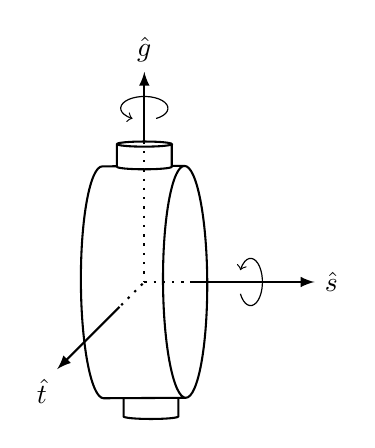
\begin{tikzpicture}[x=0.75pt,y=0.75pt,yscale=-1,xscale=1]
%uncomment if require: \path (0,284); %set diagram left start at 0, and has height of 284

%Shape: Can [id:dp7170334139971102] 
\draw  [fill={rgb, 255:red, 255; green, 255; blue, 255 }  ,fill opacity=1 ] (260.4,169.85) -- (260.4,180.76) .. controls (260.4,181.45) and (254.49,182) .. (247.2,182) .. controls (239.91,182) and (234,181.45) .. (234,180.76) -- (234,169.85) .. controls (234,169.17) and (239.91,168.62) .. (247.2,168.62) .. controls (254.49,168.62) and (260.4,169.17) .. (260.4,169.85) .. controls (260.4,170.54) and (254.49,171.09) .. (247.2,171.09) .. controls (239.91,171.09) and (234,170.54) .. (234,169.85) ;
%Shape: Can [id:dp8604613691481404] 
\draw  [color={rgb, 255:red, 0; green, 0; blue, 0 }  ,draw opacity=1 ][fill={rgb, 255:red, 255; green, 255; blue, 255 }  ,fill opacity=1 ] (263.97,171.79) -- (224.4,172.01) .. controls (218.52,172.04) and (213.61,147.06) .. (213.43,116.2) .. controls (213.26,85.35) and (217.89,60.31) .. (223.78,60.28) -- (263.34,60.06) .. controls (269.23,60.03) and (274.14,85.01) .. (274.31,115.86) .. controls (274.48,146.72) and (269.85,171.76) .. (263.97,171.79) .. controls (258.08,171.82) and (253.17,146.84) .. (253,115.98) .. controls (252.83,85.13) and (257.46,60.09) .. (263.34,60.06) ;
%Shape: Can [id:dp28656579674299] 
\draw  [fill={rgb, 255:red, 255; green, 255; blue, 255 }  ,fill opacity=1 ] (257.2,49.55) -- (257.2,60.46) .. controls (257.2,61.15) and (251.29,61.7) .. (244,61.7) .. controls (236.71,61.7) and (230.8,61.15) .. (230.8,60.46) -- (230.8,49.55) .. controls (230.8,48.87) and (236.71,48.32) .. (244,48.32) .. controls (251.29,48.32) and (257.2,48.87) .. (257.2,49.55) .. controls (257.2,50.24) and (251.29,50.79) .. (244,50.79) .. controls (236.71,50.79) and (230.8,50.24) .. (230.8,49.55) ;
%Straight Lines [id:da6813117542504483] 
\draw  [dash pattern={on 0.84pt off 2.51pt}]  (232.87,127.13) -- (244,116) ;
%Straight Lines [id:da7942658869494881] 
\draw  [dash pattern={on 0.84pt off 2.51pt}]  (244,116) -- (266,116);
%Straight Lines [id:da8094718055923082] 
\draw  [dash pattern={on 0.84pt off 2.51pt}]  (244,48.32) -- (244,116) ;

%Straight Lines [id:da10899843254419173] 
\draw[-latex]    (266,116) -- (326,116) node[anchor=west] {$\hat{s}$} node [midway] {\AxisRotator[x=0.15cm,y=0.3cm,->,rotate=0,black]} ;
%Straight Lines [id:da31922966493534966] 
\draw[-latex]    (232,128) -- (202,158) node[anchor=north east] {$\hat{t}$};
%Straight Lines [id:da6086340922936091] 
\draw[-latex]    (244,48.32) -- (244,14.71) node[above] {$\hat{g}$} node [midway] {\AxisRotator[x=0.15cm,y=0.3cm,->,rotate=90,black]};


\end{tikzpicture}
\caption{Single Gimble Control Moment Gyroscope basis vectors, initialy each SGCMG's wheel spin axis is facing towards x of pyramid, gimble axis is aligned with z axis}
\label{fig:sgcmg}
\end{figure}

\subsection{Satellite Attitude Dynamics}
\subsection{RW}
\subsection{CMG}
\subsection{VSCMG}
